\chapter*{Extra figures}
\label{ch:extra_figures}
\addcontentsline{toc}{chapter}{Extra figures}

To make the report more readable some figures are not provided directly in the text.
These figures are provided here.
We like to remind you that all of the figures from this report and many more can be found on the GitHub repository of this project \citep{github_project}.

\section*{Effect of decreasing phoneme step size}
\begin{figure*}[ht]
    \centering
    \begin{subfigure}{.45\textwidth}
        \centering
        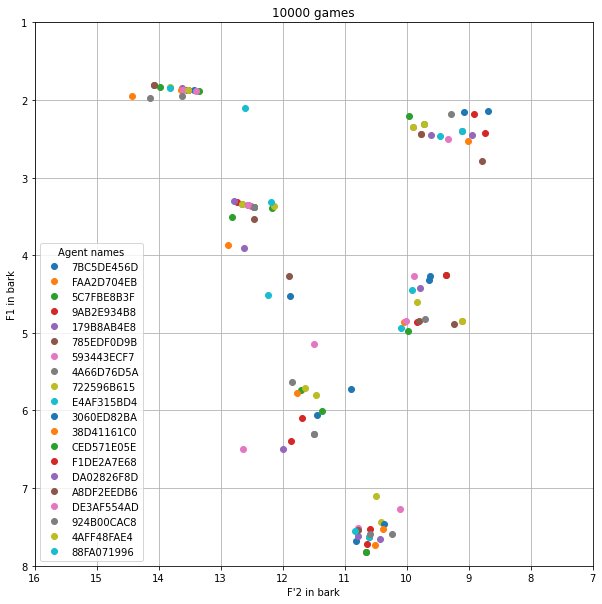
\includegraphics[width=\textwidth]{images/results/step_size_1.png}
        \captionsetup{width=0.9\linewidth}
        \captionsetup{justification=centering}
        \caption{Phoneme step size 0.1}
    \end{subfigure}
    \hspace{0.5cm}
    \begin{subfigure}{.45\textwidth}
        \centering
        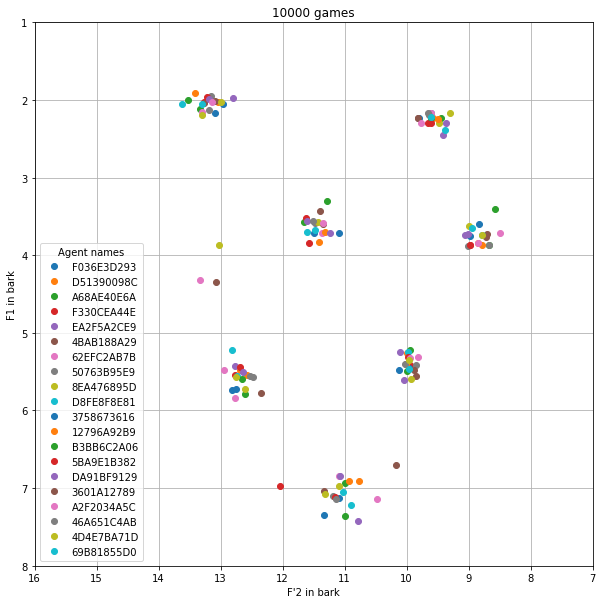
\includegraphics[width=\textwidth]{images/results/step_size_025.png}
        \captionsetup{width=0.9\linewidth}
        \captionsetup{justification=centering}
        \caption{Phoneme step size 0.025}
    \end{subfigure}
    \captionsetup{width=0.8\linewidth}
    \captionsetup{justification=centering}
    \caption{Vowel system emerged from two simulation using differing phoneme step size.}
    \label{fig:bdb_smaller_step}
\end{figure*}

\clearpage
\section*{Varying acoustic noise parameter settings for alternative bark operator}
\begin{figure*}[ht]
    \centering
    \begin{subfigure}{.30\textwidth}
        \centering
        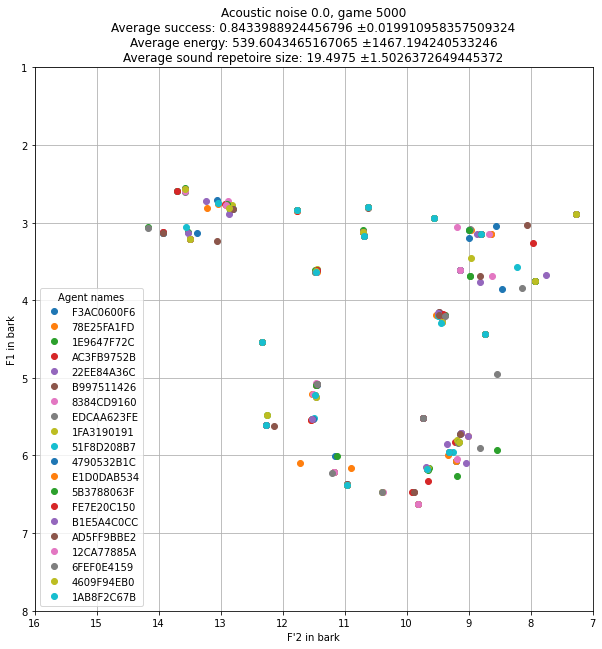
\includegraphics[width=\textwidth]{images/extra/bark_noise_1.png}
        \captionsetup{width=0.9\linewidth}
        \captionsetup{justification=centering}
        \caption{Acoustic noise = 0}
    \end{subfigure}
    \hspace{0.5cm}
    \begin{subfigure}{.30\textwidth}
        \centering
        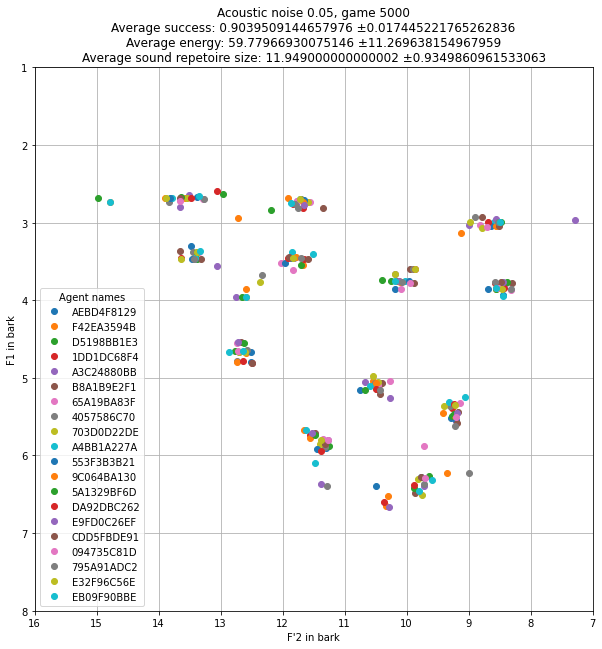
\includegraphics[width=\textwidth]{images/extra/bark_noise_2.png}
        \captionsetup{width=0.9\linewidth}
        \captionsetup{justification=centering}
        \caption{Acoustic noise = 0.05}
    \end{subfigure}
    \hspace{0.5cm}
    \begin{subfigure}{.30\textwidth}
        \centering
        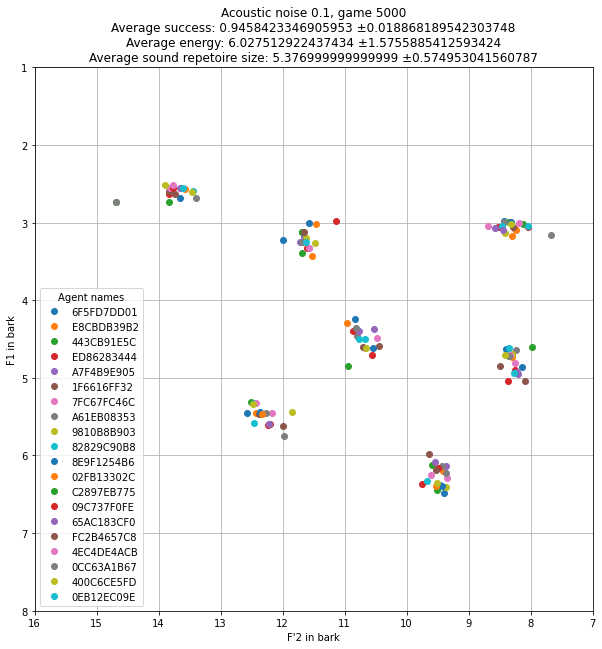
\includegraphics[width=\textwidth]{images/extra/bark_noise_3.png}
        \captionsetup{width=0.9\linewidth}
        \captionsetup{justification=centering}
        \caption{Acoustic noise = 0.1}
    \end{subfigure}
    \begin{subfigure}{.30\textwidth}
        \centering
        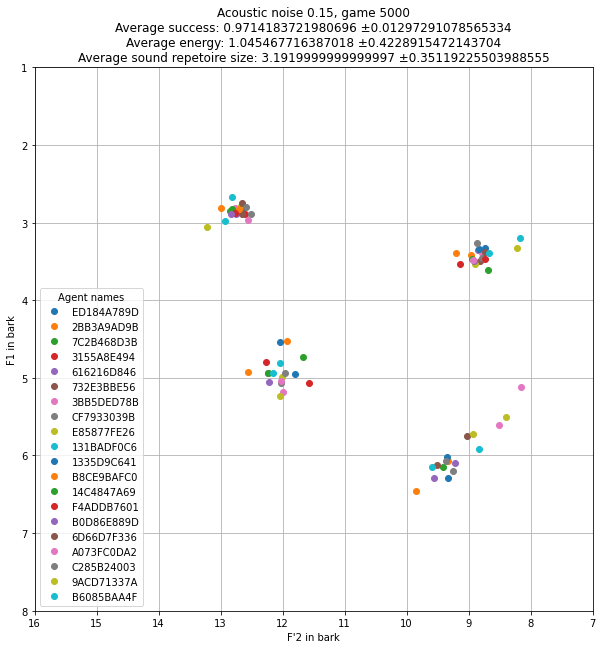
\includegraphics[width=\textwidth]{images/extra/bark_noise_4.png}
        \captionsetup{width=0.9\linewidth}
        \captionsetup{justification=centering}
        \caption{Acoustic noise = 0.15}
    \end{subfigure}
    \hspace{0.5cm}
    \begin{subfigure}{.30\textwidth}
        \centering
        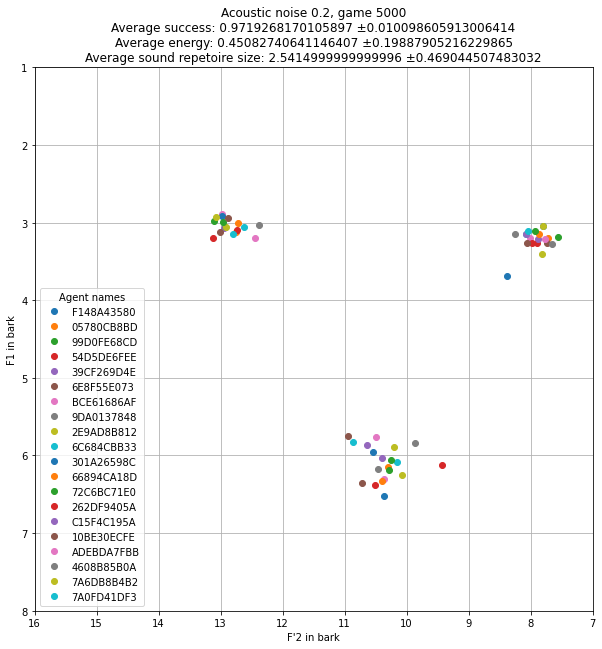
\includegraphics[width=\textwidth]{images/extra/bark_noise_5.png}
        \captionsetup{width=0.9\linewidth}
        \captionsetup{justification=centering}
        \caption{Acoustic noise = 0.2}
    \end{subfigure}
    \hspace{0.5cm}
    \begin{subfigure}{.30\textwidth}
        \centering
        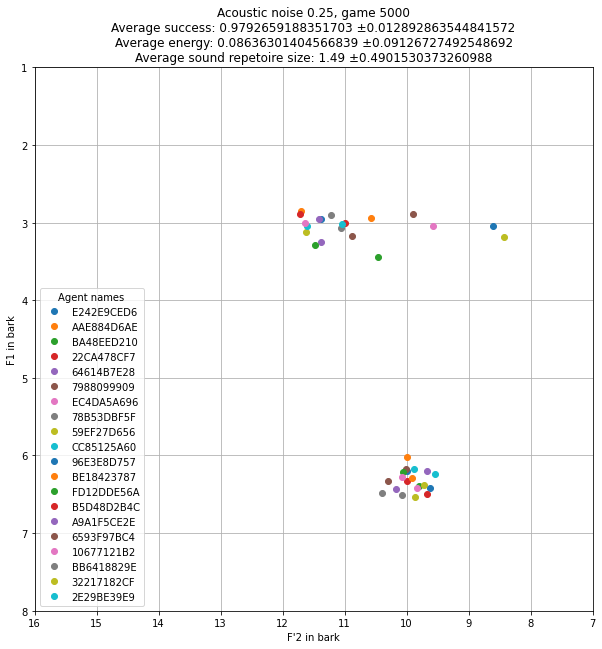
\includegraphics[width=\textwidth]{images/extra/bark_noise_6.png}
        \captionsetup{width=0.9\linewidth}
        \captionsetup{justification=centering}
        \caption{Acoustic noise = 0.25}
    \end{subfigure}
    \captionsetup{width=0.9\linewidth}
    \captionsetup{justification=centering}
    \caption{Sample games of ABM using alternative bark operator for varying acoustic noise parameters. Statistical measures are provided above each plot.}
    \label{fig:bark_noise_impact}
\end{figure*}

\clearpage
\section*{Varying effective second formant weight for alternative bark operator}
\begin{figure*}[ht]
    \centering
    \begin{subfigure}{.30\textwidth}
        \centering
        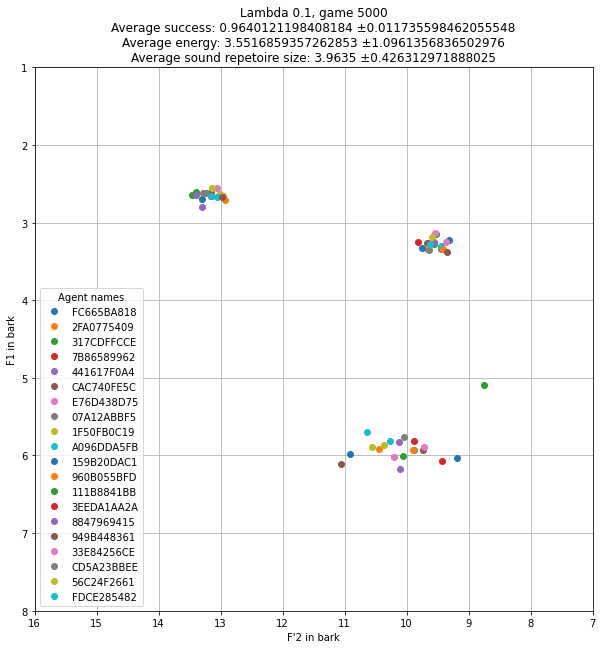
\includegraphics[width=\textwidth]{images/extra/bark_weight_1.png}
        \captionsetup{width=0.9\linewidth}
        \captionsetup{justification=centering}
        \caption{Weight = 0.1}
    \end{subfigure}
    \hspace{0.5cm}
    \begin{subfigure}{.30\textwidth}
        \centering
        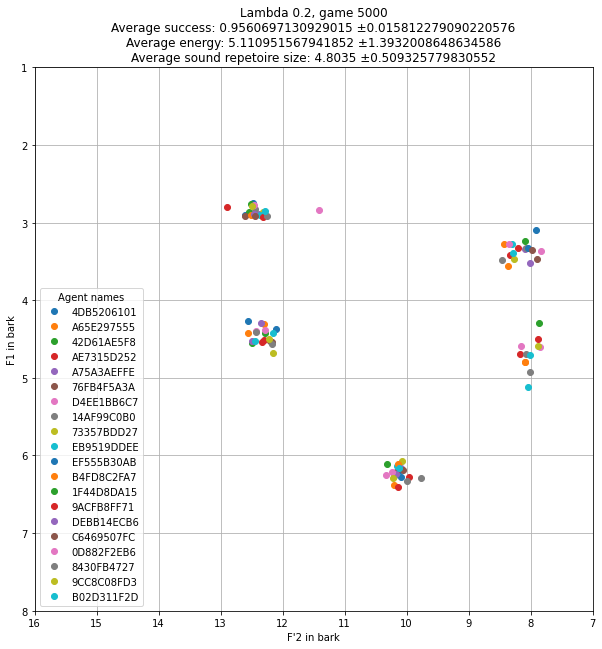
\includegraphics[width=\textwidth]{images/extra/bark_weight_2.png}
        \captionsetup{width=0.9\linewidth}
        \captionsetup{justification=centering}
        \caption{Weight = 0.2}
    \end{subfigure}
    \hspace{0.5cm}
    \begin{subfigure}{.30\textwidth}
        \centering
        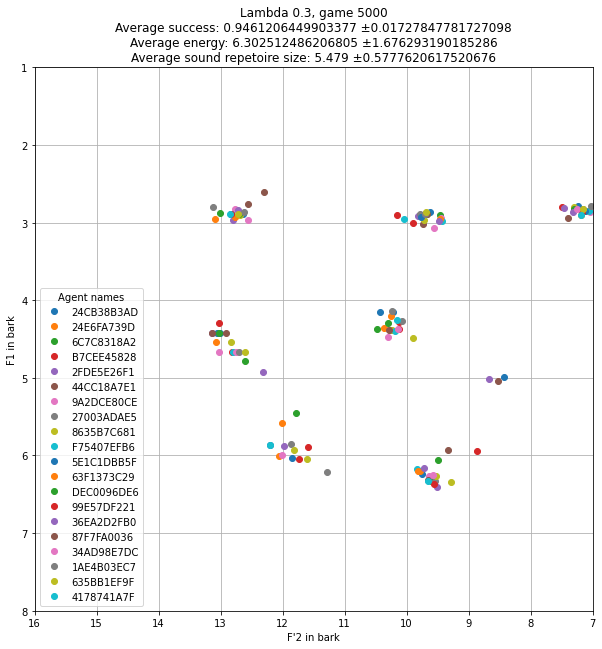
\includegraphics[width=\textwidth]{images/extra/bark_weight_3.png}
        \captionsetup{width=0.9\linewidth}
        \captionsetup{justification=centering}
        \caption{Weight = 0.3}
    \end{subfigure}
    \begin{subfigure}{.30\textwidth}
        \centering
        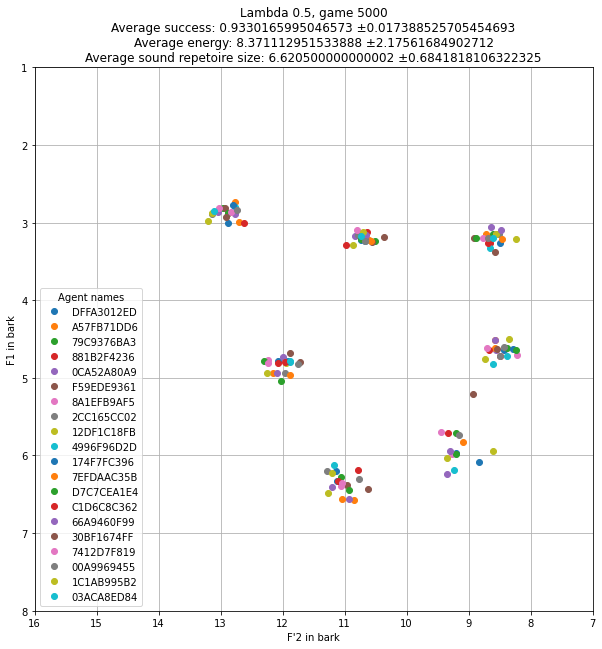
\includegraphics[width=\textwidth]{images/extra/bark_weight_4.png}
        \captionsetup{width=0.9\linewidth}
        \captionsetup{justification=centering}
        \caption{Weight = 0.5}
    \end{subfigure}
    \hspace{0.5cm}
    \begin{subfigure}{.30\textwidth}
        \centering
        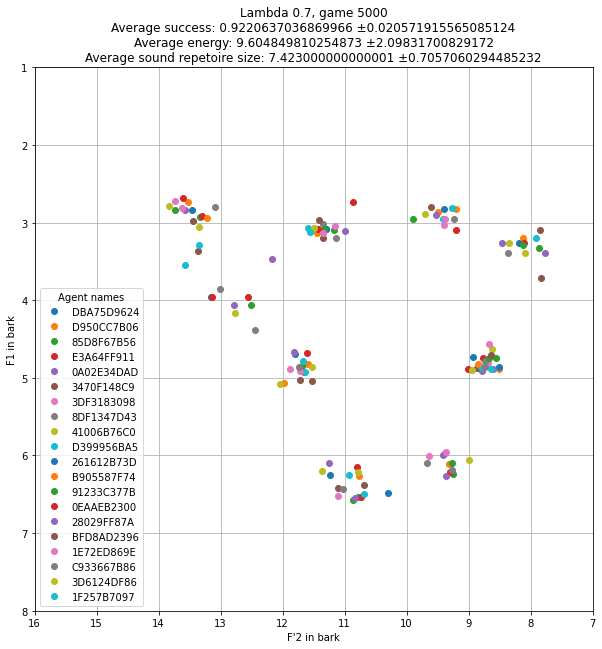
\includegraphics[width=\textwidth]{images/extra/bark_weight_5.png}
        \captionsetup{width=0.9\linewidth}
        \captionsetup{justification=centering}
        \caption{Weight = 0.7}
    \end{subfigure}
    \hspace{0.5cm}
    \begin{subfigure}{.30\textwidth}
        \centering
        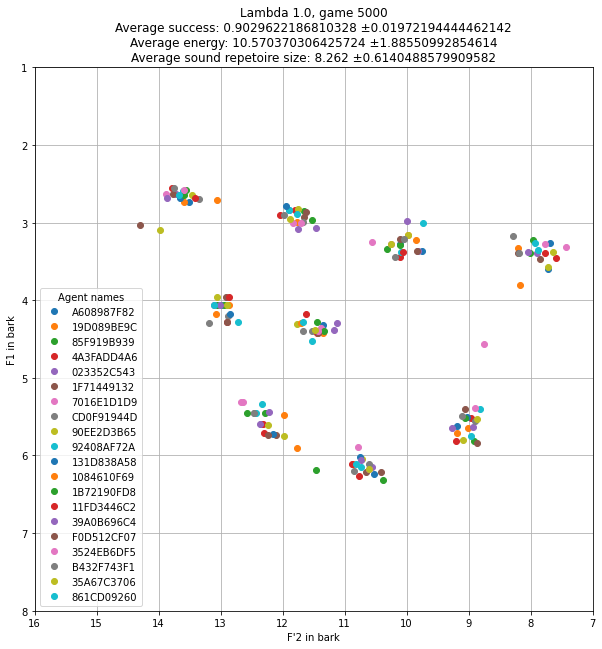
\includegraphics[width=\textwidth]{images/extra/bark_weight_6.png}
        \captionsetup{width=0.9\linewidth}
        \captionsetup{justification=centering}
        \caption{Weight = 1.0}
    \end{subfigure}
    \captionsetup{width=0.9\linewidth}
    \captionsetup{justification=centering}
    \caption{Sample games of ABM using alternative bark operator for varying effective second formant weights. Statistical measures are provided above each plot.}
    \label{fig:bark_weight_impact}
\end{figure*}

\clearpage
\section*{Overlay of known vowels}
\begin{figure}[ht]
    \centering
    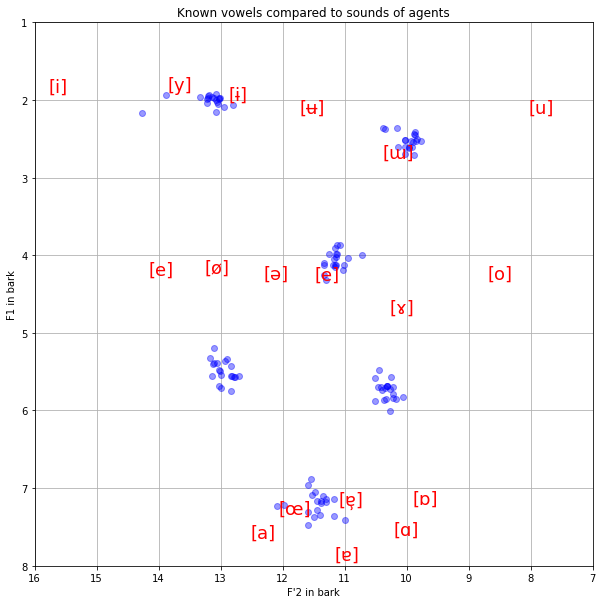
\includegraphics[width=0.6\linewidth]{images/results/overlayed_known_sounds.png}
    \captionsetup{width=\linewidth}
    \captionsetup{justification=centering}
    \caption{Overlay of known vowels on the result of a 5000 iteration imitation game.}
    \label{fig:overlayed_vowel}
\end{figure}
